In this section, we present the functional setting and some auxiliary results
for the FE discretization of the streamfunction formulation of the QGE
\eqref{eqn:QGEWF}. Let $\mathcal{T}^h$ denote a finite element triangulation of
$\Omega$ with mesh size (maximum triangle diameter) $h$. We consider a
\emph{conforming} FE discretization of \eqref{eqn:QGEWF}, i.e., let $X^h$ be
piecewise polynomials such that $X^h \subset X = H_0^2(\Omega)$.

The FE discretization of the streamfunction formulation of the QGE
\eqref{eqn:QGEWF} reads:
\begin{equation}
  \begin{split}
    &\text{Find } \psi^h \in X^h \text{ such that} \\
    \frac{\partial}{\partial t} (\nabla \psi^h, \nabla \chi^h)
      + Re^{-1} (\Delta \psi^h, \Delta \chi^h)
      &+ b(\psi^h,\psi^h,\chi^h)
      - Ro^{-1} (\psi_x^h,\chi^h)
      = Ro^{-1}(F,\chi^h),\quad \forall \, \chi^h \in X^h.
    \label{eqn:SemiDiscretization}
  \end{split}
\end{equation}
Using standard arguments \cite{Girault79,Girault86}, one can prove that, if the
small data condition used in proving the well-posedness result for the
continuous case holds, then \eqref{eqn:SemiDiscretization} has a unique solution
$\psi^h$ (see Theorem 2.1 in \cite{Cayco86}).

As noted in Section 6.1 in \cite{Ciarlet} (see also Section 13.2 in
\cite{Gunzburger89}, Section 3.1 in \cite{Johnson}, and Theorem 5.2 in
\cite{Braess}, in order to develop a conforming FE discretization for the QGE
\eqref{eqn:QGEWF}, we are faced with the problem of constructing subspaces of
the space $H^2_0(\Omega)$. Since the standard, piecewise polynomial FE spaces
are locally regular, this construction amounts in practice to finding FE spaces
$X^h$ that satisfy the inclusion $X^h \subset C^1({\bar \Omega})$, i.e., finding
$C^1$ finite elements.

Several finite elements meet this requirement (see, e.g., Section 6.1 in
\cite{Ciarlet}, Section 13.2 in \cite{Gunzburger89}, and Section 5 in
\cite{Braess}): the Argyris triangular element, the Bell triangular element, the
Hsieh-Clough-Tocher triangular element (a macroelement), and the
Bogner-Fox-Schmit rectangular element).

A description of the particular finite element we are using (the Argyris
triangle \autoref{fig:Argyris}) and its transformation will be thoroughly
discussed in \autoref{sec:Argyris}). Additionally, we note that
\eqref{eqn:SemiDiscretization} is only a semi-discretization, since the
formulation is still continuous in time, but discretized in space.  We apply the
the \emph{method of lines} (MoL) in the time domain, i.e. use a \emph{finite
difference} approximation for the time derivative.

%In what follows, we will use the Argyris triangular element, depicted in
%\autoref{fig:Argyris}.  Finite elements of class $C^1$ are of particular
%interest when employing conforming finite elements for the Steam function
%formulation of the QGE. If we are to require conforming finite elements,
%Lagrange finite elements are not enough to guarantee continuity in the first
%derivative, and so to ensure continuity in the first derivative \cite{Johnson}
%the Argyris Element (depicted in \autoref{fig:Argyris}) was implemented in our
%numerical tests. The Argyris element is probably the best known of all $C^1$
%finite elements \cite{Argyris,Dominguez06}, but appear to be rarely
%implemented.

  %\begin{figure}[h]
	\begin{center}
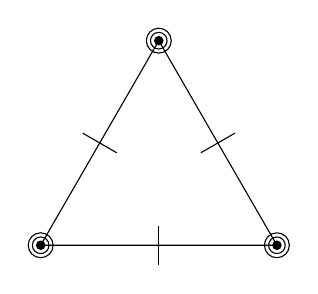
\begin{tikzpicture}[scale=0.5]
	%define the vertices of the triangle
	\path[coordinate] (0,0) coordinate(A)
		++(60:3cm) coordinate(D)
		++(60:3cm) coordinate(B)
		++(-60:3cm) coordinate(E)
		++(-60:3cm) coordinate(C)
		++(180:3cm) coordinate(F);
	%label the vertices and draw edges
	\draw (A) -- (D) -- (B) -- (E) -- (C) -- (F) -- cycle;
	%draw the interpolation points
	%function values
	\filldraw[black] (A) circle(3pt); 
	\filldraw[black] (B) circle(3pt); 
	\filldraw[black] (C) circle(3pt); 
	%first derivatives
	\draw[black] (A) circle(6pt); 
	\draw[black] (B) circle(6pt); 
	\draw[black] (C) circle(6pt); 
	%second derivatives
	\draw[black] (A) circle(9pt); 
	\draw[black] (B) circle(9pt); 
	\draw[black] (C) circle(9pt); 
	%normal derivatives
	\draw (1.067,2.848) -- (D) -- (1.933,2.348); 
	\draw (4.067,2.348) -- (E) -- (4.933,2.848); 
	\draw (3,-0.5cm) -- (F) -- (3,0.5cm); 
	%labels
%	\node[below of=A, node distance=0.5cm] (k) {$k=j+1$};
% \node[above of=B, node distance=0.5cm] (j) {$j=i+1$};
%	\node[below of=C, node distance=0.5cm] (i) {$i$};
\end{tikzpicture}
	\end{center}
	\caption{Argyris element with its 21 degrees of freedom.}
	\label{fig:Argyris}
\end{figure}

  %If we are to require conforming finite elements, Lagrange finite elements are
not enough to guarantee continuity in the first derivative, and so to ensure
continuity in the first derivative \cite{Johnson} the Argyris Element (depicted
in \autoref{fig:Argyris}) will be required. The Argyris element is probably the
best known of all $C^1$ finite elements \cite{Argyris,Dominguez08}, but appear
to be rarely implemented.

\begin{figure}[h]
	\begin{center}
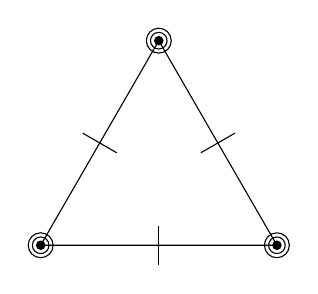
\begin{tikzpicture}[scale=0.5]
	%define the vertices of the triangle
	\path[coordinate] (0,0) coordinate(A)
		++(60:3cm) coordinate(D)
		++(60:3cm) coordinate(B)
		++(-60:3cm) coordinate(E)
		++(-60:3cm) coordinate(C)
		++(180:3cm) coordinate(F);
	%label the vertices and draw edges
	\draw (A) -- (D) -- (B) -- (E) -- (C) -- (F) -- cycle;
	%draw the interpolation points
	%function values
	\filldraw[black] (A) circle(3pt); 
	\filldraw[black] (B) circle(3pt); 
	\filldraw[black] (C) circle(3pt); 
	%first derivatives
	\draw[black] (A) circle(6pt); 
	\draw[black] (B) circle(6pt); 
	\draw[black] (C) circle(6pt); 
	%second derivatives
	\draw[black] (A) circle(9pt); 
	\draw[black] (B) circle(9pt); 
	\draw[black] (C) circle(9pt); 
	%normal derivatives
	\draw (1.067,2.848) -- (D) -- (1.933,2.348); 
	\draw (4.067,2.348) -- (E) -- (4.933,2.848); 
	\draw (3,-0.5cm) -- (F) -- (3,0.5cm); 
	%labels
%	\node[below of=A, node distance=0.5cm] (k) {$k=j+1$};
% \node[above of=B, node distance=0.5cm] (j) {$j=i+1$};
%	\node[below of=C, node distance=0.5cm] (i) {$i$};
\end{tikzpicture}
	\end{center}
	\caption{Argyris element with its 21 degrees of freedom.}
	\label{fig:Argyris}
\end{figure}


The Argyris element does, in fact, ensure $C^1$ continuity
\cite{Dominguez08,Okabe}, but at a cost of twenty-one degrees of freedom.
However, these twenty-one degrees of freedom give basis polynomials of degree
five and therefore has a very high rate of convergence \cite{Dominguez08}.
These degrees of freedom include the value at each vertex, the value of the
first derivatives at each vertex, the value of the second derivatives at each
vertex, the value of the mixed derivative at each vertex, and finally the value
of the normal derivatives at each of the edge midpoints. Here in lies the main
difficulty in implementing the Argyris triangle, the normal derivatives. Not
only do we now have 21 degrees of freedom that we must worry about, but the
added complexity of a transformation that maintains the direction of the normal
derivatives is required. Since working on the reference element is the most
common way of working with finite elements and normal derivatives are not
respected by affine transformation a more complicated transformation will have
to be employed. This is unlike a standard Lagrange element where only a simple
Affine transformation is required. \cite{Dominguez08}

Dominguez \emph{et al.} developed such a transformation. This transformation,
which is a $21 \times 21$ matrix, $C$, allows for all calculations to be done on
a reference element, vastly simplifying the calculations for the various
matrices and load vector required for the QGE finite elements calculations and
allowing for faster running code. Since, the tranformation of Dominguez is so
new and is not the standard for implementation of the Argyris element his
transformation will be discussed at length in \autoref{sse:Trans} for
completeness.

